% This LaTeX was auto-generated from MATLAB code.
% To make changes, update the MATLAB code and export to LaTeX again.

\documentclass{article}

\usepackage[utf8]{inputenc}
\usepackage[T1]{fontenc}
\usepackage{lmodern}
\usepackage{graphicx}
\usepackage{color}
\usepackage{hyperref}
\usepackage{amsmath}
\usepackage{amsfonts}
\usepackage{epstopdf}
\usepackage[table]{xcolor}
\usepackage{matlab}

\sloppy
\epstopdfsetup{outdir=./}
\graphicspath{ {./GaussQuadrDemo_images/} }

\matlabhastoc

\begin{document}

\label{T_943F305D}
\matlabtitle{Cuadraturi de tip Gauss}

\matlabtableofcontents{Cuprinsul}

\vspace{1em}

\label{H_3A3D21E2}
\matlabheading{Formule Gauss-Legendre}

\begin{par}
\begin{flushleft}
Să se calculeze integralele $\int_{-1}^1 \sin x^2 \textrm{dx}$ și $\int_{-1}^1 \cos x^2 \textrm{dx}$ cu precizia $\varepsilon =10^{-7}$ folosind o cuadratură gaussiană. Câte noduri sunt necesare?
\end{flushleft}
\end{par}

\begin{par}
\begin{flushleft}
Vom folosi o formulă de tip Gauss-Legendre
\end{flushleft}
\end{par}

\begin{matlabcode}
f1=@(x) sin(x.^2);
f2=@(x) cos(x.^2);
tol=1e-7;
n0=5;
[g_n1,g_c1]=Gauss_Legendre(n0);
v1(1)=vquad(g_n1,g_c1,f1);
v2(1)=vquad(g_n1,g_c1,f2);
k=1;
for n=n0+1:4*n0
    [gn,gc]=Gauss_Legendre(n);
    k=k+1;
    v1(k)=vquad(gn,gc,f1);
    if abs(v1(k)-v1(k-1)) < tol
        disp([gn,gc'])
        fprintf('I1(%2d)=%10.6f\n',n,v1(k))
        break;
    end
end
\end{matlabcode}
\begin{matlaboutput}
  -0.960289856497536   0.101228536290376
  -0.796666477413627   0.222381034453374
  -0.525532409916329   0.313706645877887
  -0.183434642495650   0.362683783378362
   0.183434642495650   0.362683783378362
   0.525532409916329   0.313706645877888
   0.796666477413627   0.222381034453374
   0.960289856497536   0.101228536290376
I1( 8)=  0.620537
\end{matlaboutput}
\begin{matlabcode}
k=1;
for n=n0+1:4*n0
    [gn,gc]=Gauss_Legendre(n);
    k=k+1;
    v2(k)=vquad(gn,gc,f2);
    if abs(v2(k)-v2(k-1)) < tol
        fprintf('I2(%2d)=%10.6f\n',n,v2(k))
        break;
    end
end
\end{matlabcode}
\begin{matlaboutput}
I2( 8)=  1.809048
\end{matlaboutput}

\begin{par}
\begin{flushleft}
Verificare simbolică
\end{flushleft}
\end{par}

\begin{matlabcode}
syms t rest f(t) xi
vpa(int(sin(t^2),t,-1,1))
\end{matlabcode}
\begin{matlabsymbolicoutput}
ans = 

\hskip1em $\displaystyle 0.62053660344676220361630484633079$
\end{matlabsymbolicoutput}
\begin{matlabcode}
vpa(int(cos(t^2),t,-1,1))
\end{matlabcode}
\begin{matlabsymbolicoutput}
ans = 

\hskip1em $\displaystyle 1.8090484758005441629495767336651$
\end{matlabsymbolicoutput}

\begin{par}
\begin{flushleft}
Verificare cu formula restului
\end{flushleft}
\end{par}

\begin{matlabcode}
po=legendreP(n,t);
c=coeffs(po,'All');
po=po/c(1)
\end{matlabcode}
\begin{matlabsymbolicoutput}
po = 

\hskip1em $\displaystyle \frac{7}{1287}-\frac{28\,t^2 }{143}+\frac{14\,t^4 }{13}-\frac{28\,t^6 }{15}+t^8 $
\end{matlabsymbolicoutput}
\begin{matlabcode}
rest=1/factorial(2*n)*int(po^2,t,-1,1)*subs(diff(f(t),t,n),t,xi);
[rest,vpa(rest)]
\end{matlabcode}
\begin{matlabsymbolicoutput}
ans = 

\hskip1em $\displaystyle \left(\begin{array}{cc}
\frac{7573384136472607\,\frac{\partial^8 }{\partial \xi^8 }\;f\left(\xi \right)}{3404126326545748309514119859404800} & 0.000000000000000002224765889977270125691636407827\,\frac{\partial^8 }{\partial \xi^8 }\;f\left(\xi \right)
\end{array}\right)$
\end{matlabsymbolicoutput}
\begin{matlabcode}
fplot(diff(sin(t^2),t,7),[-1,1])
\end{matlabcode}
\begin{center}
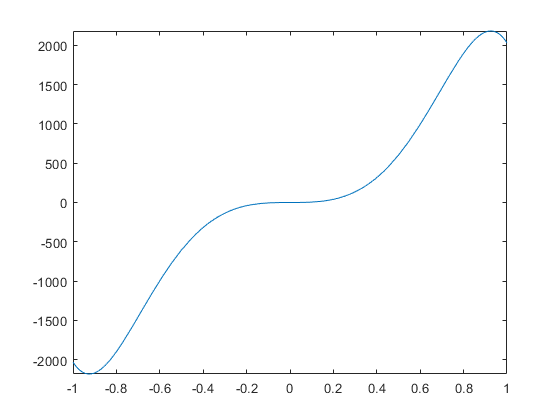
\includegraphics[width=\maxwidth{56.196688409433015em}]{figure_0.png}
\end{center}


\label{H_88A535BA}
\matlabheading{Formule Gauss-Cebîșev \#1}

\begin{par}
\begin{flushleft}
Să se aproximeze 
\end{flushleft}
\end{par}

\begin{par}
$$\int_{-1}^1 \frac{\cos \left(x\right)}{\sqrt{1-x^2 }}\textrm{dx}$$
\end{par}

\begin{par}
\begin{flushleft}
folosind o formulă gaussiană cu 10 noduri. Care este eroarea de aproximare?
\end{flushleft}
\end{par}

\begin{par}
\begin{flushleft}
Formula va fi de tip Gauss-Cebîșev de speța I. Calculăm nodurile și coeficienții. Coeficienții sunt egali cu $\frac{\pi }{10}$, iar nodurile sunt rădăcinile polinomului Cebîșev de speța 1 de grad 10, $T_n (x)=\cos (10\arccos x)$, adică $\cos \frac{(2k-1)\pi }{2n+2},~k=1..11,~n=10$.
\end{flushleft}
\end{par}

\begin{matlabcode}
[g_n,g_c]=Gauss_Cheb1(10);
disp([g_n,g_c'])
\end{matlabcode}
\begin{matlaboutput}
   0.987688340595138   0.314159265358979
   0.891006524188368   0.314159265358979
   0.707106781186548   0.314159265358979
   0.453990499739547   0.314159265358979
   0.156434465040231   0.314159265358979
  -0.156434465040231   0.314159265358979
  -0.453990499739547   0.314159265358979
  -0.707106781186547   0.314159265358979
  -0.891006524188368   0.314159265358979
  -0.987688340595138   0.314159265358979
\end{matlaboutput}

\begin{par}
\begin{flushleft}
Valoarea aproximativă a integralei este
\end{flushleft}
\end{par}

\begin{matlabcode}
format long
vI=vquad(g_n,g_c,@cos)
\end{matlabcode}
\begin{matlaboutput}
vI = 
   2.403939430634413

\end{matlaboutput}

\begin{par}
\begin{flushleft}
Deoarece $\left|\cos^{\left(n\right)} x\right|\le 1$, restul va fi mai mic decât
\end{flushleft}
\end{par}

\begin{matlabcode}
po=chebyshevT(10,t)/2^(9)
\end{matlabcode}
\begin{matlabsymbolicoutput}
po = 

\hskip1em $\displaystyle -\frac{1}{512}+\frac{25\,t^2 }{256}-\frac{25\,t^4 }{32}+\frac{35\,t^6 }{16}-\frac{5\,t^8 }{2}+t^{10} $
\end{matlabsymbolicoutput}
\begin{matlabcode}
rest=1/factorial(20)*int(po^2/sqrt(1-t^2),t,-1,1)
\end{matlabcode}
\begin{matlabsymbolicoutput}
rest = 

\hskip1em $\displaystyle \frac{8536795713241637\,\pi }{10889035741470030830827987437816582766592}$
\end{matlabsymbolicoutput}
\begin{matlabcode}
double(vpa(rest))
\end{matlabcode}
\begin{matlaboutput}
ans = 
     2.462948541511184e-24

\end{matlaboutput}

\begin{par}
\begin{flushleft}
Putem face și o verificare simbolică. Valoarea exactă a integralei este
\end{flushleft}
\end{par}

\begin{matlabcode}
ve=int(cos(t)/sqrt(1-t^2),t,-1,1)
\end{matlabcode}
\begin{matlabsymbolicoutput}
ve = 

\hskip1em $\displaystyle \pi \,{{\textrm{J}}}_0 \left(1\right)$
\end{matlabsymbolicoutput}

\begin{par}
\begin{flushleft}
Diferența dintre valoarea exactă și cea calculată:
\end{flushleft}
\end{par}

\begin{matlabcode}
double(ve)
\end{matlabcode}
\begin{matlaboutput}
ans = 
   2.403939430634413

\end{matlaboutput}
\begin{matlabcode}
abs(double(ve)-vI)
\end{matlabcode}
\begin{matlaboutput}
ans = 
     4.440892098500626e-16

\end{matlaboutput}

\begin{par}
\begin{flushleft}
Explicați de ce este mai mare decât restul.
\end{flushleft}
\end{par}


\label{H_822E222B}
\matlabheading{Formule Gauss-Cebîșev \#2}

\begin{par}
\begin{flushleft}
Să se aproximeze 
\end{flushleft}
\end{par}

\begin{par}
$$\int_{-1}^1 \sqrt{1-x^2 }\cos \left(x\right)\textrm{dx}$$
\end{par}

\begin{par}
\begin{flushleft}
folosind o formulă gaussiană cu 5 noduri. Care este eroarea de aproximare?
\end{flushleft}
\end{par}

\begin{par}
\begin{flushleft}
Formula va fi de tip Gauss-Cebîșev de speța II. Calculăm nodurile și coeficienții. Nodurile sunt rădăcinile polinomului Cebîșev de speța II de grad 5, $U_n (x)=\frac{\sin (n+1)\arccos (x)}{\sqrt{1-x^2 }}$.
\end{flushleft}
\end{par}

\begin{matlabcode}
[g_n,g_c]=Gauss_Cheb2(5);
disp([g_n,g_c'])
\end{matlabcode}
\begin{matlaboutput}
  -0.866025403784439   0.130899693899575
  -0.500000000000000   0.392699081698724
  -0.000000000000000   0.523598775598299
   0.500000000000000   0.392699081698724
   0.866025403784439   0.130899693899575
\end{matlaboutput}

\begin{par}
\begin{flushleft}
Valoarea aproximativă a integralei este
\end{flushleft}
\end{par}

\begin{matlabcode}
format long
vI=vquad(g_n,g_c,@cos)
\end{matlabcode}
\begin{matlaboutput}
vI = 
   1.382459687798957

\end{matlaboutput}

\begin{par}
\begin{flushleft}
Deoarece $\left|\cos^{\left(n\right)} x\right|\le 1$, restul va fi mai mic decât
\end{flushleft}
\end{par}

\begin{matlabcode}
po=chebyshevU(5,t)/2^5
\end{matlabcode}
\begin{matlabsymbolicoutput}
po = 

\hskip1em $\displaystyle \frac{3\,t}{16}-t^3 +t^5 $
\end{matlabsymbolicoutput}
\begin{matlabcode}
rest=1/factorial(10)*int(po^2*sqrt(1-t^2),t,-1,1)
\end{matlabcode}
\begin{matlabsymbolicoutput}
rest = 

\hskip1em $\displaystyle \frac{1301357606610903\,\pi }{9671406556917033397649408}$
\end{matlabsymbolicoutput}
\begin{matlabcode}
double(vpa(rest))
\end{matlabcode}
\begin{matlaboutput}
ans = 
     4.227239825522600e-10

\end{matlaboutput}

\begin{par}
\begin{flushleft}
Putem face și o verificare simbolică. Valoarea exactă a integralei este
\end{flushleft}
\end{par}

\begin{matlabcode}
ve=int(cos(t)*sqrt(1-t^2),t,-1,1)
\end{matlabcode}
\begin{matlabsymbolicoutput}
ve = 

\hskip1em $\displaystyle \pi \,{{\textrm{J}}}_1 \left(1\right)$
\end{matlabsymbolicoutput}

\begin{par}
\begin{flushleft}
Diferența dintre valoarea exactă și cea calculată:
\end{flushleft}
\end{par}

\begin{matlabcode}
double(ve)
\end{matlabcode}
\begin{matlaboutput}
ans = 
   1.382459687384169

\end{matlaboutput}
\begin{matlabcode}
abs(double(ve)-vI)
\end{matlabcode}
\begin{matlaboutput}
ans = 
     4.147882037841555e-10

\end{matlaboutput}

\begin{par}
\begin{flushleft}
Ea este în concordanță cu restul.
\end{flushleft}
\end{par}


\label{H_577FA4C5}
\matlabheading{Formule Gauss-Laguerre}

\begin{par}
\begin{flushleft}
Să se aproximeze 
\end{flushleft}
\end{par}

\begin{par}
$$\int_0^{\infty } e^{-x} \sin \left(x\right)\textrm{dx}$$
\end{par}

\begin{par}
\begin{flushleft}
folosind o formulă gaussiană cu 6 noduri. Care este eroarea de aproximare?
\end{flushleft}
\end{par}

\begin{par}
\begin{flushleft}
Formula este de tip Gauss-Laguerre.
\end{flushleft}
\end{par}

\begin{par}
\begin{flushleft}
Nodurile formulei vor fi rădăcinile polinomului Laguerre de grad 6, ortogonal pe $(0,\infty )$ în raport cu ponderea $w(x)=e^{-x}$.
\end{flushleft}
\end{par}

\begin{matlabcode}
po=laguerreL(6,0,t)
\end{matlabcode}
\begin{matlabsymbolicoutput}
po = 

\hskip1em $\displaystyle 1-6\,t+\frac{15\,t^2 }{2}-\frac{10\,t^3 }{3}+\frac{5\,t^4 }{8}-\frac{t^5 }{20}+\frac{t^6 }{720}$
\end{matlabsymbolicoutput}
\begin{matlabcode}
c=coeffs(po,'All');
po=po/c(1)
\end{matlabcode}
\begin{matlabsymbolicoutput}
po = 

\hskip1em $\displaystyle 720-4320\,t+5400\,t^2 -2400\,t^3 +450\,t^4 -36\,t^5 +t^6 $
\end{matlabsymbolicoutput}

\begin{par}
\begin{flushleft}
Coeficienții și nodurile se obțin astfel
\end{flushleft}
\end{par}

\begin{matlabcode}
[g_n,g_c]=Gauss_Laguerre(6);
disp([g_n,g_c'])
\end{matlabcode}
\begin{matlaboutput}
   0.222846604179261   0.458964673949964
   1.188932101672623   0.417000830772121
   2.992736326059315   0.113373382074045
   5.775143569104513   0.010399197453149
   9.837467418382587   0.000261017202815
  15.982873980601699   0.000000898547906
\end{matlaboutput}

\begin{par}
\begin{flushleft}
Valoarea integralei
\end{flushleft}
\end{par}

\begin{matlabcode}
format long
vI=vquad(g_n,g_c,@sin)
\end{matlabcode}
\begin{matlaboutput}
vI = 
   0.500049474797675

\end{matlaboutput}

\begin{par}
\begin{flushleft}
Deoarece $\left|\sin^{\left(n\right)} x\right|\le 1$, restul va fi mai mic decât
\end{flushleft}
\end{par}

\begin{matlabcode}
rest=1/factorial(12)*int(po^2*exp(-t),t,0,Inf)
\end{matlabcode}
\begin{matlabsymbolicoutput}
rest = 

\hskip1em $\displaystyle \frac{1277696559217977675}{1180591620717411303424}$
\end{matlabsymbolicoutput}
\begin{matlabcode}
double(vpa(rest))
\end{matlabcode}
\begin{matlaboutput}
ans = 
   0.001082251082251

\end{matlaboutput}

\begin{par}
\begin{flushleft}
Putem face și o verificare simbolică. Valoarea exactă a integralei este
\end{flushleft}
\end{par}

\begin{matlabcode}
ve=int(sin(t)*exp(-t),t,0,Inf)
\end{matlabcode}
\begin{matlabsymbolicoutput}
ve = 

\hskip1em $\displaystyle \frac{1}{2}$
\end{matlabsymbolicoutput}

\begin{par}
\begin{flushleft}
Diferența dintre valoarea exactă și cea calculată:
\end{flushleft}
\end{par}

\begin{matlabcode}
double(ve)
\end{matlabcode}
\begin{matlaboutput}
ans = 
   0.500000000000000

\end{matlaboutput}
\begin{matlabcode}
abs(double(ve)-vI)
\end{matlabcode}
\begin{matlaboutput}
ans = 
     4.947479767514196e-05

\end{matlaboutput}

\begin{par}
\begin{flushleft}
Ea este în concordanță cu restul.
\end{flushleft}
\end{par}


\label{H_8F953890}
\matlabheading{Formule Gauss-Hermite}

\begin{par}
\begin{flushleft}
Să se aproximeze
\end{flushleft}
\end{par}

\begin{par}
$$\int_{-\infty }^{\infty } e^{-x^2 } \left(\cos \left(x\right)+\sin \left(x\right)\right)\textrm{dx}$$
\end{par}

\begin{par}
\begin{flushleft}
cu 8 zecimale exacte.
\end{flushleft}
\end{par}

\begin{par}
\begin{flushleft}
Formula este de tip Gauss-Hermite. Vom obține numărul de noduri din formula restului. Derivata de orice ordin a lui $\cos x+\sin x$ este $\le \sqrt{2}$
\end{flushleft}
\end{par}

\begin{matlabcode}
syms R
for n=5:15
    po=hermiteH(n,t);
    c=coeffs(po,'All');
    po=po/c(1);
    R=int(po^2*exp(-t^2),t,-Inf,Inf)/factorial(2*n);
    if double(R) < 1e-8/sqrt(2)
        po, R 
        disp([double(R),n])
        break
    end
end
\end{matlabcode}
\begin{matlabsymbolicoutput}
po = 

\hskip1em $\displaystyle -\frac{105\,t}{8}+\frac{105\,t^3 }{4}-\frac{21\,t^5 }{2}+t^7 $
R = 

\hskip1em $\displaystyle \frac{\sqrt{\pi }}{2214051840}$
\end{matlabsymbolicoutput}
\begin{matlaboutput}
   0.000000000800548   7.000000000000000
\end{matlaboutput}

\begin{par}
\begin{flushleft}
Calculăm nodurile, coeficienții și valoarea aproximativă a integralei
\end{flushleft}
\end{par}

\begin{matlabcode}
f=@(x) sin(x)+cos(x);
[g_n,g_c]=Gauss_Hermite(n);
disp([g_n,g_c'])
\end{matlabcode}
\begin{matlaboutput}
  -2.651961356835232   0.000971781245100
  -1.673551628767471   0.054515582819127
  -0.816287882858965   0.425607252610128
   0.000000000000000   0.810264617556807
   0.816287882858964   0.425607252610128
   1.673551628767471   0.054515582819127
   2.651961356835233   0.000971781245100
\end{matlaboutput}
\begin{matlabcode}
vI=vquad(g_n,g_c,f)
\end{matlabcode}
\begin{matlaboutput}
vI = 
   1.380388447754078

\end{matlaboutput}

\begin{par}
\begin{flushleft}
Valoarea exactă a integralei
\end{flushleft}
\end{par}

\begin{matlabcode}
ve=int(exp(-t^2)*(cos(t)+sin(t)),t,-Inf,Inf)
\end{matlabcode}
\begin{matlabsymbolicoutput}
ve = 

\hskip1em $\displaystyle \sqrt{\pi }\,{\mathrm{e}}^{-\frac{1}{4}} $
\end{matlabsymbolicoutput}
\begin{matlabcode}
abs(double(ve)-vI)
\end{matlabcode}
\begin{matlaboutput}
ans = 
     7.109348665323978e-10

\end{matlaboutput}

\begin{par}
\begin{flushleft}
este în concordanță cu restul.
\end{flushleft}
\end{par}


\label{H_A0A37FBD}
\matlabheading{Formule Gauss-Jacobi}

\begin{par}
\begin{flushleft}
Să se aproximeze
\end{flushleft}
\end{par}

\begin{par}
$$\int_{-1}^1 \sqrt{\frac{1-x}{1+x}}\frac{x^2 }{1+x^2 }\textrm{dx}$$
\end{par}

\begin{par}
\begin{flushleft}
folosind o formulă gaussiană cu 8 noduri. Care este eroarea de aproximare?
\end{flushleft}
\end{par}

\begin{par}
\begin{flushleft}
Formula este de tip Gauss-Jacobi.
\end{flushleft}
\end{par}

\begin{par}
\begin{flushleft}
Nodurile formulei vor fi rădăcinile polinomului Jacobi de grad 8, ortogonal pe $[-1,1]$ în raport cu ponderea $w(x)=\sqrt{\frac{1-x}{1+x}}$.
\end{flushleft}
\end{par}

\begin{matlabcode}
po=jacobiP(8,1/2,-1/2,t);
c=coeffs(po,'All');
po=po/c(1)
\end{matlabcode}
\begin{matlabsymbolicoutput}
po = 

\hskip1em $\displaystyle \frac{1}{256}-\frac{t}{32}-\frac{5\,t^2 }{32}+\frac{5\,t^3 }{16}+\frac{15\,t^4 }{16}-\frac{3\,t^5 }{4}-\frac{7\,t^6 }{4}+\frac{t^7 }{2}+t^8 $
\end{matlabsymbolicoutput}

\begin{par}
\begin{flushleft}
Coeficienții și nodurile se obțin astfel
\end{flushleft}
\end{par}

\begin{matlabcode}
[g_n,g_c]=Gauss_Jacobimodificat(8,1/2,-1/2);
disp([g_n,g_c'])
\end{matlabcode}
\begin{matlaboutput}
  -0.982973099683902   0.732905143792132
  -0.850217135729614   0.683838654253425
  -0.602634636379256   0.592332376475014
  -0.273662990072083   0.470744740324667
   0.092268359463302   0.335496829804836
   0.445738355776538   0.204854624665768
   0.739008917220659   0.096462078624944
   0.932472229404356   0.024958205649009
\end{matlaboutput}

\begin{par}
\begin{flushleft}
Valoarea integralei
\end{flushleft}
\end{par}

\begin{matlabcode}
f=@(x) x.^2./(1+x.^2);
format long
vI=vquad(g_n,g_c,f)
\end{matlabcode}
\begin{matlaboutput}
vI = 
   0.920152566416141

\end{matlaboutput}

\begin{par}
\begin{flushleft}
Valoarea exactă a integralei
\end{flushleft}
\end{par}

\begin{matlabcode}
ve=int(sqrt((1-t)/(1+t))*t^2/(1+t^2),t,-1,1)
\end{matlabcode}
\begin{matlabsymbolicoutput}
ve = 

\hskip1em $\displaystyle -\frac{\pi \,{\left(\sqrt{2}-2\right)}}{2}$
\end{matlabsymbolicoutput}
\begin{matlabcode}
abs(double(ve)-vI)
\end{matlabcode}
\begin{matlaboutput}
ans = 
     1.381905530672967e-06

\end{matlaboutput}

\begin{par}
\begin{flushleft}
este în concordanță cu valoarea calculată.
\end{flushleft}
\end{par}

\begin{par}
\begin{flushleft}
Restul va fi
\end{flushleft}
\end{par}

\begin{matlabcode}
syms f(t) F(t)
f(t)=t^2/(1+t^2);
R=int(po^2*sqrt((1-t)/(1+t)),t,-1,1)/factorial(16)*subs(diff(F(t),t,16),t,xi)
\end{matlabcode}
\begin{matlabsymbolicoutput}
R = 

\hskip1em $\displaystyle \frac{\pi \,\frac{\partial^{16} }{\partial \xi^{16} }\;F\left(\xi \right)}{1371195958099968000}$
\end{matlabsymbolicoutput}
\begin{matlabcode}
double(int(po^2*sqrt((1-t)/(1+t)),t,-1,1)/factorial(16))
\end{matlabcode}
\begin{matlaboutput}
ans = 
     2.291133251255364e-18

\end{matlaboutput}
\begin{matlabcode}
fplot(diff(f(t),t,16),[-1,1])
\end{matlabcode}
\begin{center}
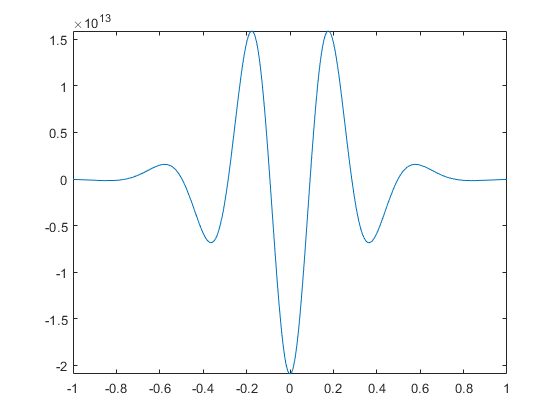
\includegraphics[width=\maxwidth{56.196688409433015em}]{figure_1.png}
\end{center}

\begin{par}
\begin{flushleft}
Valoarea aproximativă a restului va fi
\end{flushleft}
\end{par}

\begin{matlabcode}
R=int(po^2*sqrt((1-t)/(1+t)),t,-1,1)/factorial(16)*subs(diff(f(t),t,16),t,0)
\end{matlabcode}
\begin{matlabsymbolicoutput}
R = 

\hskip1em $\displaystyle -\frac{\pi }{65536}$
\end{matlabsymbolicoutput}
\begin{matlabcode}
double(R)
\end{matlabcode}
\begin{matlaboutput}
ans = 
    -4.793689962142629e-05

\end{matlaboutput}

\end{document}
